\begin{frame}{Aufgabe}
	\begin{itemize}
		\item Webserver für Most Useless Machine Ever!
	\end{itemize}
	\begin{center}
		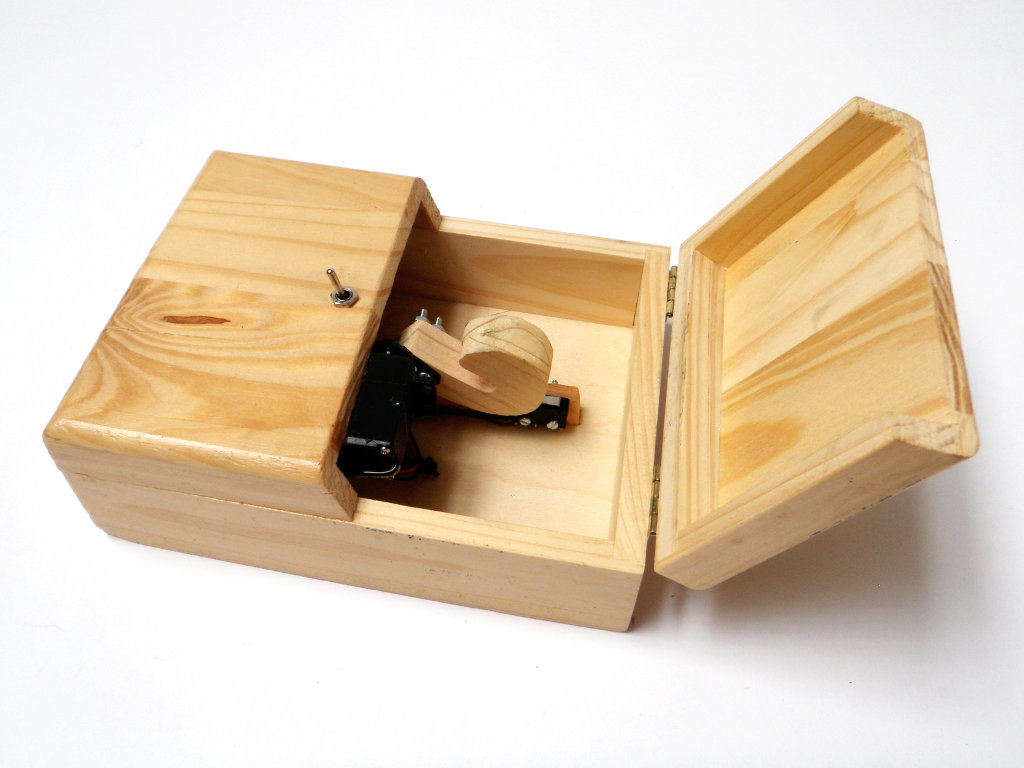
\includegraphics[width=0.75\textwidth]{res/mume.jpg}
		\cite{mumePic}
	\end{center}
\end{frame}

\begin{frame}{System}
	\begin{itemize}
		\item uC oder GNU/Linux?
		\item uC wie Arduino
		\begin{itemize}
			\item Echtzeit
			\item niedrige System-Komplexität
			\item keine Infrastruktur
		\end{itemize}
		\item GNU/Linux
		\begin{itemize}
			\item Treiber
			\item Protokolle
			\item Memory und Prozess Management
			\item hohe System-Komplexität
		\end{itemize}
	\end{itemize}
\end{frame}

\begin{frame}{Hardware}
	\begin{itemize}
		\item Eval-/Bastelboards (Raspi, BeagleBone)
		\item Consumer Hardware (Router, Media-Center, \ldots)
		\item Profesionelle Boards
		\item[$\rightarrow$] BeagleBone Green
		\begin{itemize}
			\item Netzwerk
			\item USB
			\item Yocto Supported
			\item viele Anshlüsse
			\item USB Powered
			\item kein Display Anschluss
			\item bereits Erfahrung
		\end{itemize}
	\end{itemize}
\end{frame}

\begin{frame}{GNU/Linux Distribution}
	\begin{itemize}
		\item Yocto\cite{whyYocto} \footnote{Tools und Rezepte um eigene GNU/Linux Distribution zu bauen}
		\begin{itemize}
			\item git repository mit Konfiguration des gesamten System
			\item Patches einzelner Pakete
			\item Optimierungen für spezifische Hardware
			\item volle Kontrolle
		\end{itemize}
		\item off-the-shelf (Debian, Arch, Gentoo, Ubuntu)
		\begin{itemize}
			\item weite Verbreitung; bekannt
			\item Updates werden von anderen bereitgestellt
			\item erlaubt Lizenz Verteilung?
		\end{itemize}
	\end{itemize}
\end{frame}
